\chapter{模型验证及实验结果分析}
\label{chap:exp}

在实验中,我们利用CPU集群和多块Xeon Phi针对模型及其多种并行实现方法进行了运行时间,扩展性测试,
以及最优化的参数设置调试。我们的测试将先从单块的Xeon Phi Knight Corner处理器和Xeon E52670(Sandybridge)处理器开始,用它们来测试我们的单块并行算法
Omp1和Omp2,我们的测试集中在两个方面,一是对比算法在CPU平台和Xeon Phi平台上的表现;二是测试和比较两种算法的优, 
并利用6块Xeon Phi Knight Corner来进行我们的扩展性测试。最后我们利用\textsl{Maison de la Simulation}的CPU集群\textsl{Poincare}
来测试我们的算法收敛性。
% \begin{table}[htbp]
% \caption{Xeon Phi 参数列表}
% \label{tab:MIC}
% \centering
% \resizebox{\linewidth}{!}{\footnotesize
% 	\begin{tabular}{|c|c|c|c|c|} 
% 	\hline
% 	\hline
% 	\end{tabular}
% \end{table}
\section{单块Xeon Phi和CPU的实验对比} % (fold)
\label{sec:singleMIC-CPU}
单块Xeon Phi的并行方案是多块Xeon Phi并行方案的基础,同时单块Xeon Phi方案的性能依赖于参数的
选取。我们的实验将给出重要参数的优化取值范围,同时通过与相同代码在CPU下地性能对比来验证
Xeon Phi架构对我们的模型的重要性。

\subsection{单机并行方案一的实验} % (fold)
\label{sub:bsV1}
单机并行方案中最重要的参数是Ncache值和Chunck值的选取(见算法\ref{alg:omp1}),
Ncache的取值大小将影响缓存的效率,而Chunck值的选取则会影响不同的线程任务分配方案。
我们首先测试在不给定Chunck值(采用系统自己的线程任务分配方案)时Ncache值对算法的影响。
在图\ref{fig:v1-chunck-Ncache} 中,我们
在X轴上选取不同的Ncache值,同时给出5组选取不同Chunck值的时间曲线。该测试中得时间均为没做一次蒙特卡洛模拟的平均时间。
为了缩短测试时间,我们取蒙特卡洛模拟的次数较小($M=10$),这就会使我们的测试时间有一定的波动性,因为蒙特卡洛模拟具有随机的性质。但是
从趋势上来看,我们仍然可以给出分析结果。
\begin{figure}[!t]
   \centering
   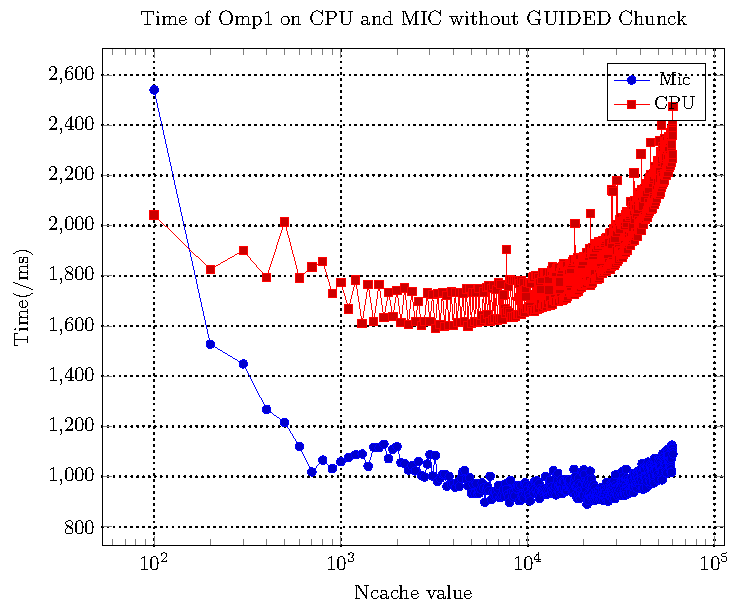
\includegraphics[width=\textwidth]{chap5/Figures/bsV1-6-mic-cpu-Time-Chunck-0.pdf}
   \caption{算法Omp1在不同Ncache值下的运行时间, $N=10^6$, $M=10$, 图中Omp1的运行时间随着Ncache的值先降低后增加,表明Ncache有一个
   最佳的取值范围。图中也可以看出同样地参数下算法在Xeon Phi平台上表现得比CPU平台下更好。由于M的取值较小,曲线具有一定的波动性。}
   \label{fig:v1-Ncache}
\end{figure}

我们发现算法在Xeon Phi上的表现优于CPU上的表现,并且当$10^4 < Ncache < 10^5$时,算法\ref{alg:omp1}在CPU和Xeon Phi上都存在一个最优化时间的窗口, 
这分别对应了CPU和Xeon Phi上的缓存大小,只有当
每次任务所需内存接近这个缓存大小时才能充分发挥性能。当我们考察Chunck值对算法的影响时,我们从图
\ref{fig:v1-mic-chunck-Ncache} \ref{fig:v1-cpu-chunck-Ncache} 中可以看到,取不同的Chunck值,
对算法的性能并没有明显的影响。
\begin{figure}[!t]
   \centering
   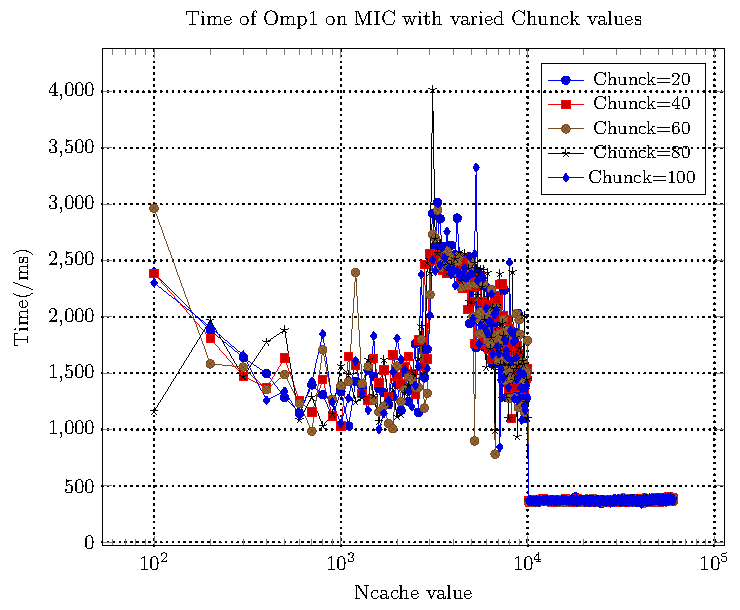
\includegraphics[width=\textwidth]{chap5/Figures/bsV1-mic-Time-Chunck.pdf}
   \caption{算法Omp1在MIC以及不同Chunck值下的时间, $N=10^5$, $M=10$, 图中当Ncache小于$10^4$时,各种Chunck值对应的曲线都有随机波动,但是
   并没有明显的优劣之分,而当$Ncache > 10^4$时,不同Chunck值的曲线都收敛在一起。}
   \label{fig:v1-mic-chunck-Ncache}
\end{figure}
这可以理解为,当一块Xeon Phi或者CPU上面的所有线程同时工作于一块Ncache大小的缓存区域时,每次分配给单个线程的任务量并不影响总的运算时间。
\begin{figure}[!t]
   \centering
   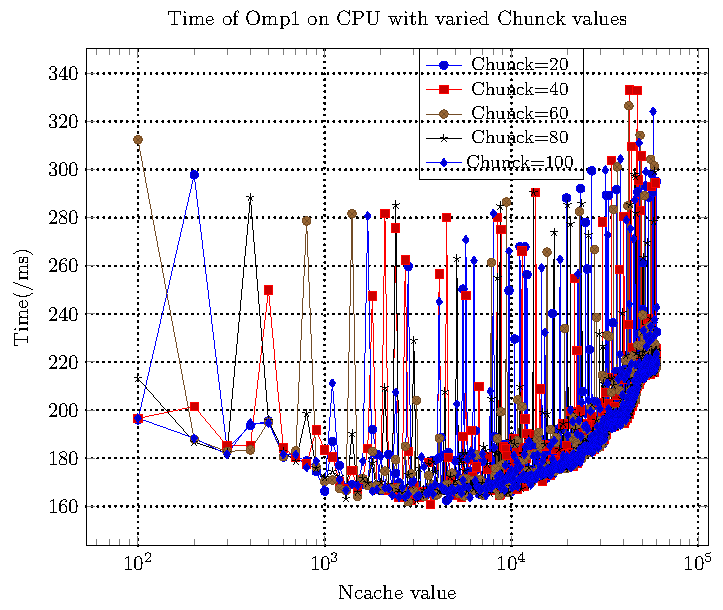
\includegraphics[width=\textwidth]{chap5/Figures/bsV1-CPU-Time-Chunck.pdf}
   \caption{算法Omp1在CPU以及不同Chunck值下运行时间对比, $N=10^5$, $M=10$, 图中的曲线出现较大的波动性,不同的Chunck值对应的曲线之间
   也没有明显的优劣,但所有的曲线都有一个明显的总体趋势,即有一个Ncache的最佳取值范围获得最好的性能}
   \label{fig:v1-cpu-chunck-Ncache}
\end{figure}
据此,我们可以直接利用系统自己智能非配的线程任务策略,而不同自己人为设定Chunck的大小。
\subsection{单机并行方案二的实验} % (fold)
\label{sub:bsV2}
在第二种单机并行方案中同样有两个重要的可调节参数,Nvec和Chunck值的大小(见算法\ref{alg:omp2})
同样的,我们先使用系统自己的线程任务分配机制(不设置Chunck值)。图\label{fig:v2-Nvec}中显示
算法在Xeon Phi上的性能优于CPU上的性能,并且当Nvec取值在500左右时可以使Xeon Phi发挥出最好的性能。
\begin{figure}[!t]
   \centering
   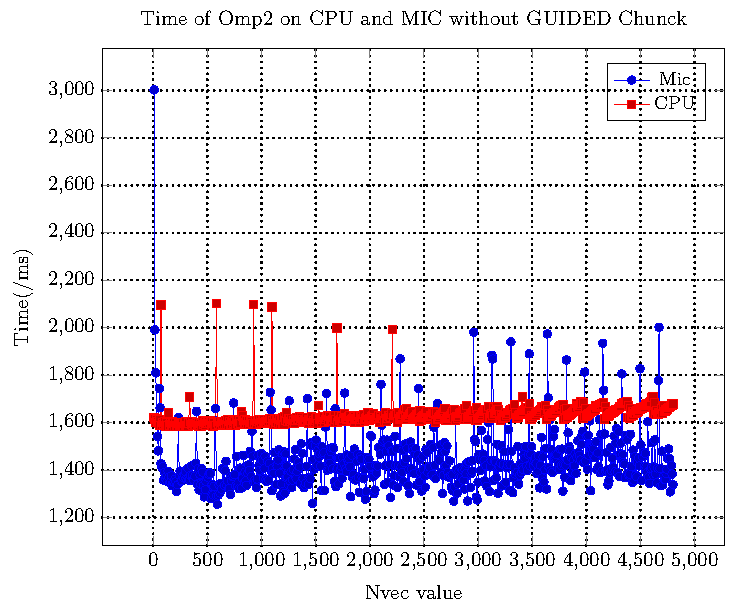
\includegraphics[width=\textwidth]{chap5/Figures/bsV2-6-mic-cpu-Time-Chunck-0.pdf}
   \caption{算法Omp2在不同Nvec值下的运行时间, $N=10^6$, $M=10$, CPU所代表的红色曲线波动性较小,随着Nvec的值也无明显变化,说明系统在默认的
   Chunck策略下自动进行了调整;同样Xeon Phi所代表的蓝色曲线虽然比红色曲线波动更大,但是总体趋势也是稳定在一个较优的性能上。}
   \label{fig:v2-Nvec}
\end{figure}
图\ref{fig:v2-mic-chunck-Nvec},\ref{fig:v2-cpu-chunck-Nvec}则反映出了取不同的Chunck值对性能的影响。当Nvec的值大于$10^3$后,计算速度
迅速下降,因为分配给单个核的内存任务超过了核本身的缓存大小,在这种情况下,取较小的Chunck的值可以获得相对理想的性能,因为这样单个核分配到的任务较小,
缓存对速度的影响较小。
\begin{figure}[!t]
   \centering
   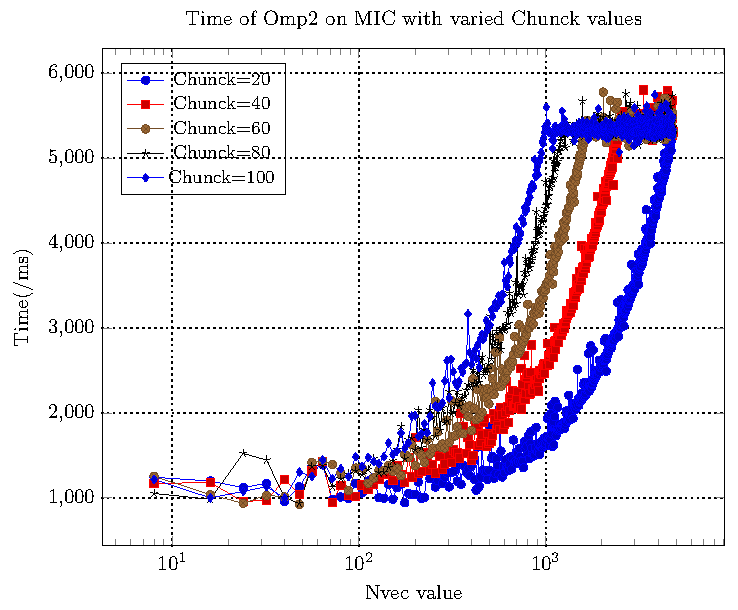
\includegraphics[width=\textwidth]{chap5/Figures/bsV2-mic-Time-Chunck.pdf}
   \caption{算法Omp2在MIC以及不同Chunck值下的时间, $N=10^5$, $M=10$, 可以明显地看到不同的曲线在Nvec的值大于100后出现了分离,较小值的Chunck策略
   获得了更好地性能,这是由于较小的单个线程任务量减弱了Nvec值超出单个核缓存造成的性能降低;而当Nvec的取值较小时不同的Chunck取值无明显区别。}
   \label{fig:v2-mic-chunck-Nvec}
\end{figure}
而当Nvec的值较小时,每个线程都能充分利用核上的缓存从而获得好的计算速度,而这时Chunck对性能的影响就很小了,我们在以后的实验中采用系统默认的Chunck方案,
或者Chunck为1的方案。
\begin{figure}[!t]
   \centering
   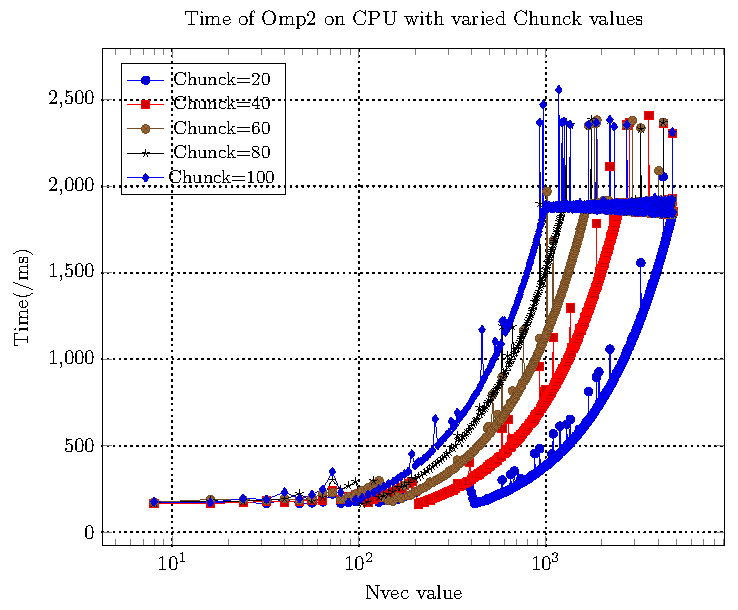
\includegraphics[width=\textwidth]{chap5/Figures/bsV2-CPU-Time-Chunck.pdf}
   \caption{算法Omp2在CPU以及不同Chunck值下运行时间对比, $N=10^5$, $M=10$}
   \label{fig:v2-cpu-chunck-Nvec}
\end{figure}

\subsection{两种单机并行方案的对比} % (fold)
\label{sub:compareV1V2}

在测试了我们的两种单机并行方案后,我们发现Xeon Phi能更好地发挥我们算法的性能。所以在对比两种算法优劣时,我们选择在Xeon Phi平台上进行测试。
图\label{fig:compareV1V2}对比了两种方案在Xeon Phi平台上不同OpenMP线程数下相对串行算法的加速比。
\begin{figure}[!t]
   \centering
   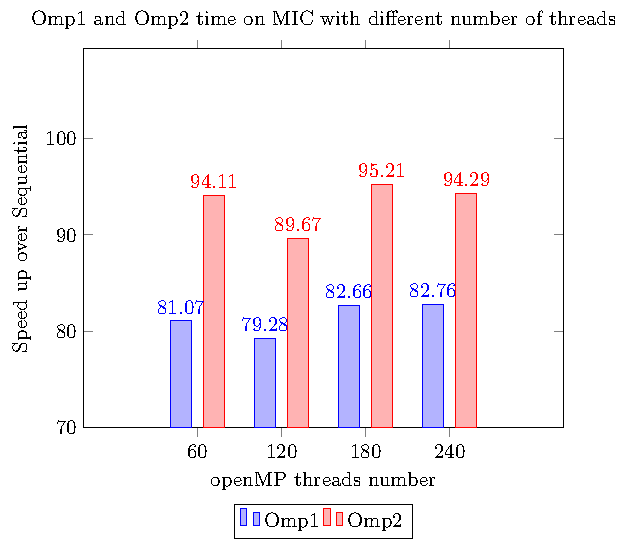
\includegraphics[width=\textwidth]{chap5/Figures/BS-Core-bar.pdf}
   \caption{Omp1, Omp2相对串行算法在MIC上的加速对比, Chunck 采用系统默认模式, $N=251988$, $M=100$, $Ncache=2000$, $Nvec=376$}
   \label{fig:compareV1V2}
\end{figure}
我们看到算法\ref{alg:omp2}明显优于算法\ref{alg:omp1}。算法\ref{alg:omp2}最大的加速比达到来了95倍。同时算法\ref{alg:omp1}在Xeon Phi 平台上也获得了
不错的加速比(80x)。考察单块Xeon Phi上的线程数对性能的影响,我们发现我们的算法在采用不同线程数(单核1线程,2线程,3线程和4线程)时性能的差别不是
很显著。主要原因是我们调优了两种算法的参数Ncache 和 Nvec。对于算法\ref{alg:omp1}来说,因为所有的数据都存储在Xeon Phi的缓存区,所以线程总数的改变
不会显著影响性能;对于算法\ref{alg:omp2}, 通过前面的分析,我们采用一个较小的Nvec值,可以使单个线程的任务装进单个核的缓存中,即使线程数量增加,也能
较好地发挥缓存的作用。

\section{多块Xeon Phi的并行结果分析} % (fold)
\label{sec:multiMIC}
在之前的分析基础上,我们认为算法\ref{alg:omp2}的表现优于算法\ref{alg:omp1}, 同时Xeon Phi平台的表现优于CPU平台。在这一小节中我们就要测试和分析
算法\ref{alg:omp2}在多个Xeon Phi环境下的严格扩展性(Strong Scalability)。受限制与实验设备,我们的Xeon Phi测试平台只有6块Xeon Phi处理器,并且
Xeon Phi处理器之间的连接速度并不理想。根据Pingpang测试的结果,我们发现两块Xeon Phi之间的通信速度只有307Mbyte/s,
但是由图\ref{fig:scale}中可知,我们的算法获得了超线性(superlinear)的扩展性。
\begin{figure}[!t]
   \centering
   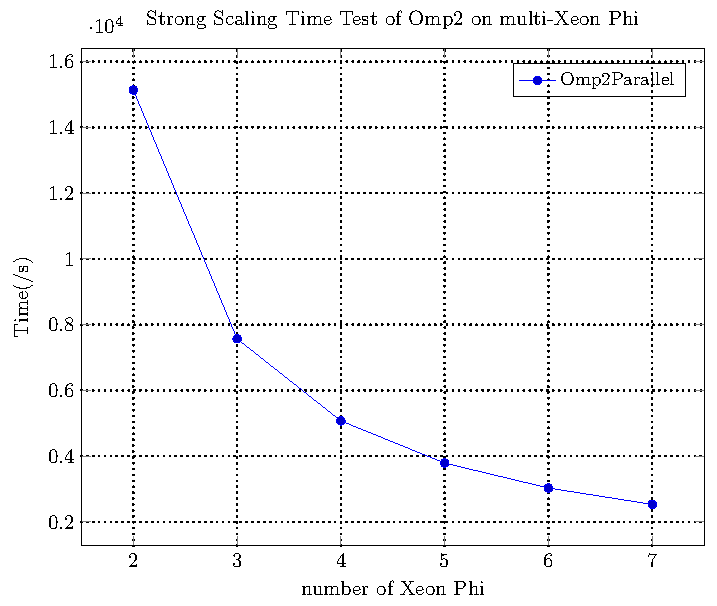
\includegraphics[width=\textwidth]{chap5/Figures/bsmpi-mic-scale.pdf}
   \caption{Omp2Parallel在multi-Xeon Phi上运行时间的严格扩展性$N=251988$, $M=10000$, $Ncache=2000$, $Nvec=192$。图中显示我们的算法
	   获得了超线性的扩展性能,这种超线性扩展的结果部分是由于我们的算法所基于的蒙特卡洛模拟。首先蒙特卡洛模拟需要大量的计算量来达到收敛性,
		   是个计算密集型的算法,其次蒙特卡洛各次模拟之间具有相互独立性,给算法上的实现提供了很大的潜在并行性。
		   同时我们的并行算法让单块Xeon Phi只负责一次蒙特卡洛的循环,这样各个Xeon Phi之间由于蒙特卡洛的独立性从而只有极小部分的通信需求,
		   这就使算法获得了非常理想的扩展性。}
   \label{fig:scale}
\end{figure}
这种超线性扩展的结果部分是由于我们的算法所基于的蒙特卡洛模拟。首先蒙特卡洛模拟需要大量的计算量来达到收敛性,是个计算密集型的算法,其次蒙特卡洛
各次模拟之间具有相互独立性,给算法上的实现提供了很大的潜在并行性。同时我们的并行算法让单块Xeon Phi只负责一次蒙特卡洛的循环,这样各个Xeon Phi之间
由于蒙特卡洛的独立性从而只有极小部分的通信需求, 这就使算法获得了非常理想的扩展性。

\section{算法的收敛性研究} % (fold)
\label{sec:converge}
我们模型和算法的最外层是通过二分法来搜索最小的符合条件的$N$值。通过增加蒙特卡洛模拟的次数$M$, 我们可以使搜索到得$N$值逐渐收敛到一个准确地值。
收敛性的测试是在一个有92个节点,184块Xeon E5的集群上进行测试。因为我们目前可供使用的Xeon Phi数量有限(6块),而收敛性测试所需要的$M$值
很大($10^6$), 我们才选择在CPU集群上进行测试。另一方面,我们的收敛性测试验证的是我们的算法,和运行平台无关,这也是我们选择CPU集群的原因。
图\ref{fig:converge}中显示当我们的$M$次数超过$10^4$,我们搜索到得$N$值已经收敛。而且整个收敛过程中,我们算法的效果随着$M$值的增大也未表现出
很大的波动性。
\begin{figure}[!t]
   \centering
   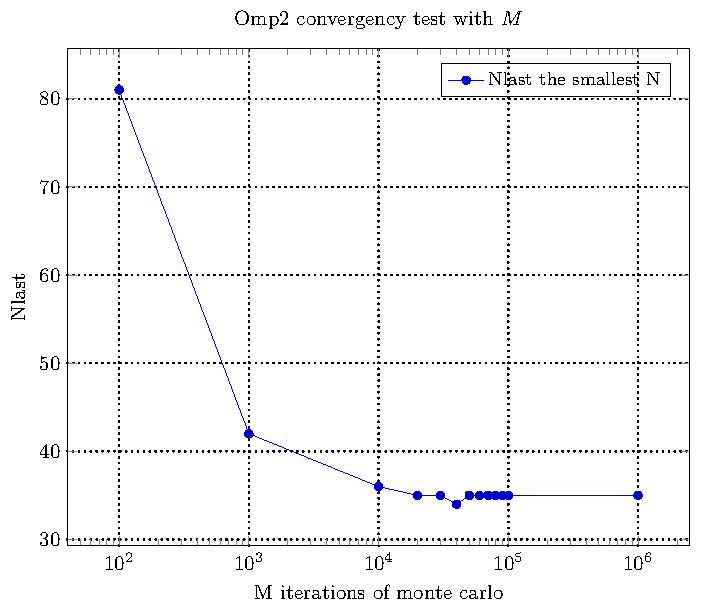
\includegraphics[width=\textwidth]{chap5/Figures/bs-converge.pdf}
   \caption{Omp2Parallel在multi-CPU上的收敛性, $N=251988$, $Nvec=192$ 当我们的$M$次数超过$10^4$,我们搜索到得$N$值已经收敛。
	   而且整个收敛过程中,我们算法的效果随着$M$值的增大也未表现出很大的波动性。}
   \label{fig:converge}
\end{figure}
这种良好的收敛性质使得我们的并行扩展性获得了意义,只要并行更多地处理器,就可以快速地收敛到我们所需要的$N$值。










